\documentclass[../mathNotesPreamble]{subfiles}

\providecommand{\relscalefact}{1.4}
\begin{document}
\relscale{\relscalefact}
  \section{9.1: Sample Means of Random Samples}
%    \textbf{Recall:} Sample statistics and population parameters are represented using different symbols \hspace*{\stretch{1}} (English for statistics, Greek for population): \hspace*{\stretch{1}}
    \begin{center}
      \begin{tabular}{@{}*{2}{lr}@{}}\toprule
        \multicolumn{2}{@{}l}{Statistics} & \multicolumn{2}{l}{Parameters} \\\midrule
        Sample mean & $\overline{x}$ & Population mean & $\mu$ \\
        Sample standard deviation & $s$ & Population standard deviation & $\sigma$\\
        Sample proportion & $\hat{p}$ & Population proportion & $p$\\\bottomrule
      \end{tabular}
    \end{center}
    \vspace*{\stretch{1}}

    \begin{defn*}
      \begin{itemize}
        \item The \textbf{sampling distribution} is the distribution of the sample means $\bar{x}$.
        \item The mean of the sampling distribution is $\mu$ so the statistic $\bar{x}$ is an \textbf{unbiased estimator}.
        \item The standard deviation of the sampling distribution is the \textbf{standard error}:
          \[SE=\frac{\sigma}{\sqrt{n}}\]
      \end{itemize}
    \end{defn*}
    \vspace*{\stretch{1}}
%    \pagebreak

    \begin{center}
      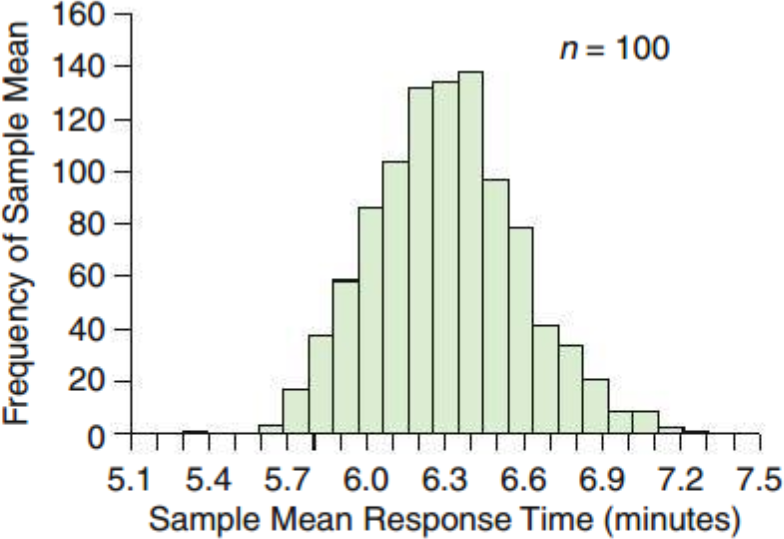
\includegraphics[width=0.3\linewidth]{images/math211_figure_9p3a}\hfill
      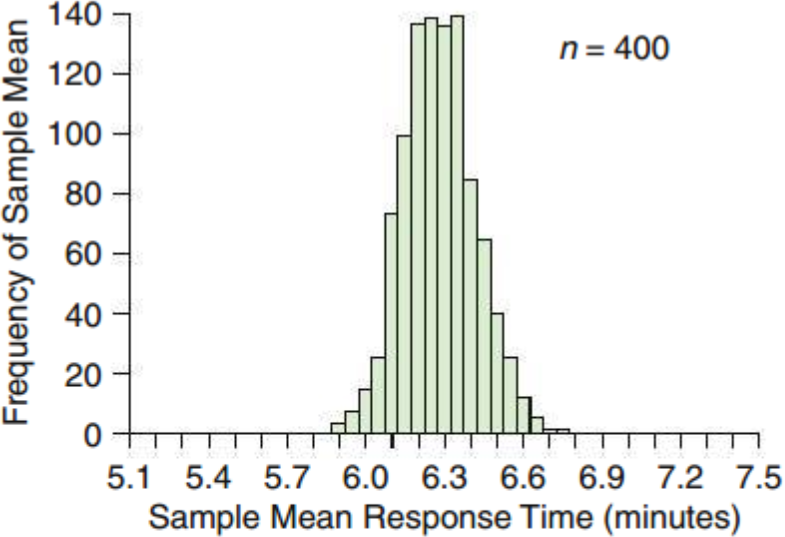
\includegraphics[width=0.3\linewidth]{images/math211_figure_9p3b}\hfill
      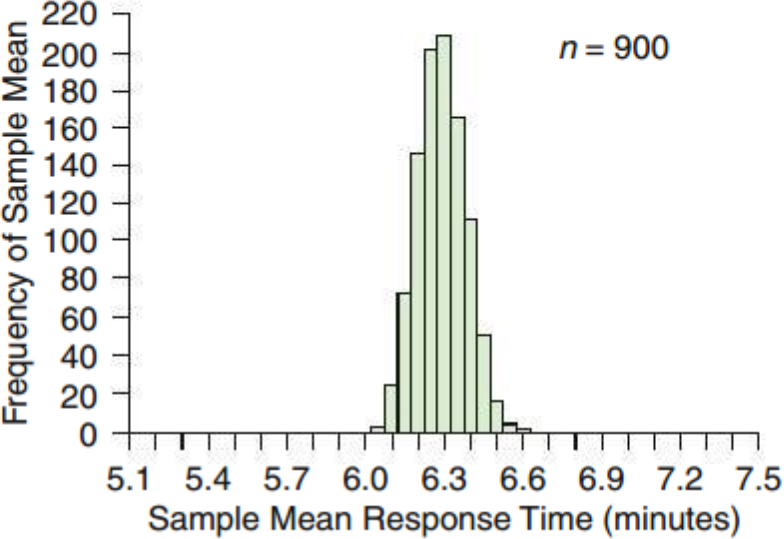
\includegraphics[width=0.3\linewidth]{images/math211_figure_9p3c}
    \end{center}

  \pagebreak
\end{document}
